\documentclass[11pt]{article}

\usepackage[margin=1in]{geometry}
\usepackage{amsmath,amssymb,amsthm}
\usepackage{mathrsfs}
\usepackage{enumitem}
\usepackage{graphicx}
\usepackage[hidelinks]{hyperref}

\newtheorem{theorem}{Theorem}
\newtheorem{lemma}{Lemma}
\newtheorem{proposition}{Proposition}

\newcommand{\B}{\mathscr{B}}
\newcommand{\G}{\mathscr{G}}
\newcommand{\K}{\mathscr{K}}
\newcommand{\F}{\mathscr{F}}
\newcommand{\SZ}{\mathscr{S\!Z}}
\newcommand{\Id}{I}
\newcommand{\cnull}{c_0}
\newcommand{\C}{C}
\newcommand{\Ker}{\operatorname{Ker}}
\newcommand{\Sz}{\operatorname{Sz}}

\title{A Conditional Low-Szlenk Reduction for the SHAI Problem on \(C[0,\omega^\omega]\)}
\author{arXiv automatic math run \texttt{fa\_banach\_001}}
\date{Candidate conditional packet, June 14, 2026}

\begin{document}
\maketitle

\section*{Classification}

\begin{itemize}[leftmargin=2em]
\item \textbf{Status:} conditional reduction.
\item \textbf{Source:} B. Horvath and T. Kania,
\emph{Surjective homomorphisms from algebras of operators on long sequence
spaces are automatically injective}, arXiv:2007.14112.
\item \textbf{Target:} Question 3.26 asks whether \(C(K)\) has the SHAI
property for \(K=[0,1]\), \(K=[0,\omega^\omega]\),
\(K=\beta\mathbb N\setminus\mathbb N\), and \(K=\beta\Gamma\) for an
uncountable discrete space \(\Gamma\).
\item \textbf{Scope of this packet:} only the subcase
\(X=C[0,\omega^\omega]\), and only conditional on one operator-ideal
equality.
\end{itemize}

\section*{Source Question}

The source question appears on PDF page 20, in Question 3.26.

\begin{center}
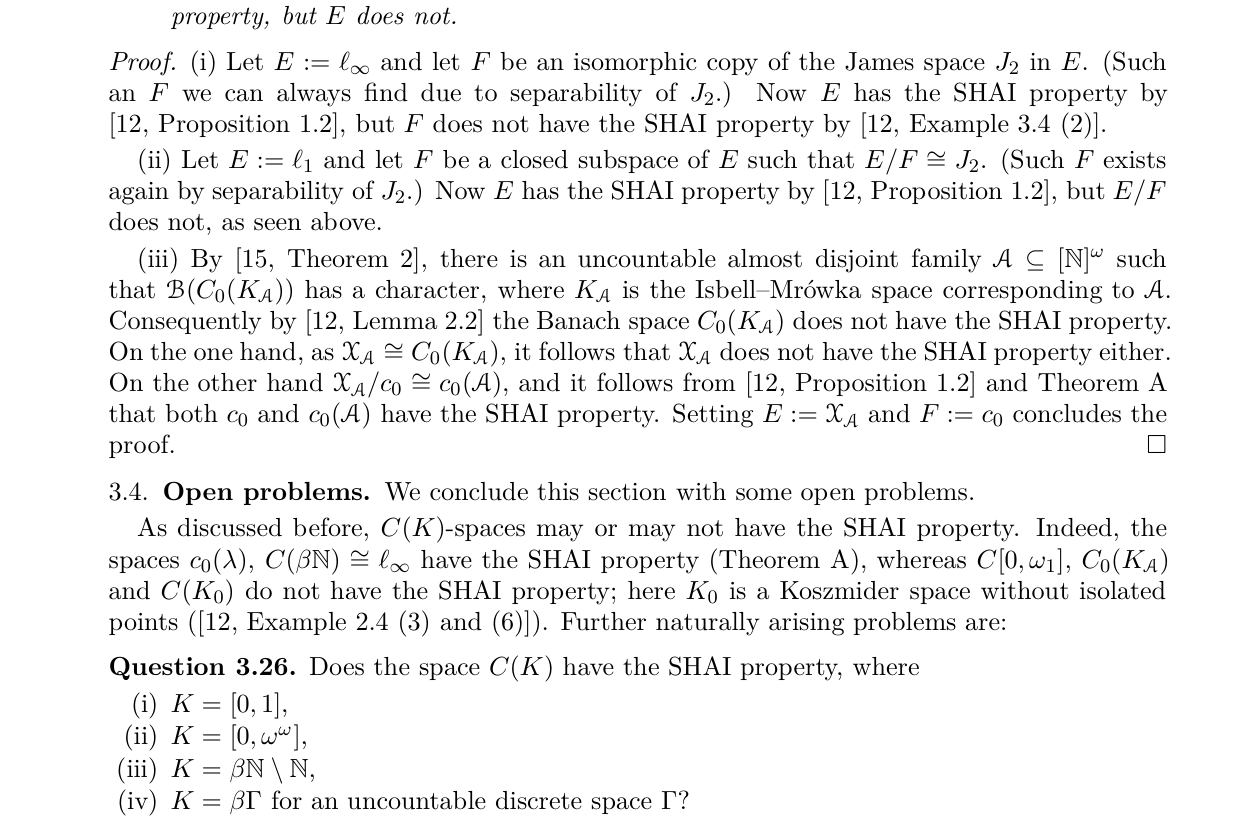
\includegraphics[width=\linewidth]{figures/open_problem_page20_question326.png}
\end{center}

\section*{Conditional Dependencies}

Let
\[
X=C[0,\omega^\omega],
\qquad
J=\overline{\G}_{\cnull}(X),
\]
where \(J\) is the closed ideal of operators on \(X\) which are norm limits
of operators factoring through \(c_0\).  Let
\[
\SZ_1(X)=\{T\in\B(X): \Sz(T)\leq \omega\}
\]
be the first Szlenk operator ideal restricted to \(\B(X)\).

This packet assumes the following unproved dependency.

\begin{description}[leftmargin=2em]
\item[(D)] \(J=\SZ_1(X)\).
\end{description}

Equivalently, every operator on \(C[0,\omega^\omega]\) with Szlenk index at
most \(\omega\) is a norm limit of operators factoring through \(c_0\).
The packet does \emph{not} prove (D).

\section*{Proof Intuition}

Horvath--Kania already prove that every non-injective SHAI quotient of
\(\B(C(K))\) kills \(\overline{\G}_{c_0}(C(K))\).  Thus, for
\(X=C[0,\omega^\omega]\), the problem is to understand what remains after
quotienting by \(J\).

Assumption (D) turns \(J\) into the boundary between small and large
operators.  If \(T\notin J\), then \(\Sz(T)>\omega\).  Bourgain's theorem,
combined with Pe\l{}czynski's complementation theorem, then forces the
identity on \(X\) to factor through \(T\).  Hence every operator outside
\(J\) generates the whole algebra \(\B(X)\), so \(J\) is a maximal ideal.
The source kernel containment now says that a non-injective quotient
\(\B(X)\to\B(Y)\) must have kernel \(J\), making \(\B(Y)\) simple.  This is
impossible for infinite-dimensional \(Y\) because of the finite-rank ideal,
and finite-dimensional \(Y\) is excluded by the square property of
\(C[0,\omega^\omega]\).

\section*{Conditional Theorem}

\begin{theorem}
Assume (D).  Then \(C[0,\omega^\omega]\) has the SHAI property.
\end{theorem}

\begin{proof}
Set \(X=C[0,\omega^\omega]\) and \(J=\overline{\G}_{c_0}(X)\).

First we show that \(J\) is a maximal two-sided ideal of \(\B(X)\).  Let
\(T\in\B(X)\setminus J\).  By (D), \(T\notin \SZ_1(X)\), so
\(\Sz(T)>\omega\).  The Bourgain theorem quoted in Kania--Laustsen says that
if an operator \(T:C(K)\to E\) has Szlenk index exceeding \(\omega^\alpha\),
then \(T\) fixes an isomorphic copy of
\(C[0,\omega^{\omega\cdot\alpha}]\).  Taking \(\alpha=1\), \(K=[0,\omega^\omega]\),
and \(E=X\), we find a subspace \(W\subseteq X\), \(W\cong X\), such that
\(T|_W\) is bounded below.

The range \(T[W]\) is a closed subspace of the separable space \(X\) and is
isomorphic to \(C[0,\omega^\omega]\).  By Pe\l{}czynski's complementation
theorem, \(T[W]\) contains a further closed subspace \(Z\cong X\) which is
complemented in \(X\).  Passing to the inverse image of \(Z\) inside \(W\),
the elementary factorization criterion gives operators \(A,B\in\B(X)\) such
that
\[
A T B=\Id_X.
\]
Thus the two-sided ideal generated by \(T\) is all of \(\B(X)\).  Since this
holds for every \(T\notin J\), every proper two-sided ideal of \(\B(X)\) is
contained in \(J\).  Hence \(J\) is maximal, and \(\B(X)/J\) is simple.

Now let \(Y\neq 0\) be a Banach space and let
\[
\psi:\B(X)\longrightarrow \B(Y)
\]
be a surjective algebra homomorphism.  Suppose, toward a contradiction, that
\(\psi\) is not injective.  Horvath--Kania Corollary 4.7 gives
\[
J=\overline{\G}_{c_0}(X)\subseteq \Ker\psi.
\]
The kernel is proper because \(\psi\) is surjective onto the nonzero unital
algebra \(\B(Y)\).  By maximality of \(J\), \(\Ker\psi=J\).  Hence
\[
\B(Y)\cong \B(X)/J
\]
is simple.

If \(Y\) is infinite-dimensional, this is impossible: the finite-rank
operators \(\F(Y)\) form a nonzero proper two-sided ideal of \(\B(Y)\).
If \(Y\) is finite-dimensional, then \(\Ker\psi\) has finite codimension in
\(\B(X)\).  But \(X=C[0,\omega^\omega]\) is isomorphic to its square, and
Horvath's finite-dimensional reduction lemma for SHAI spaces with a
complemented square records that \(\B(X)\) has no proper finite-codimensional
ideals.  This is again impossible.

Therefore no non-injective surjective homomorphism \(\B(X)\to\B(Y)\) exists,
which is exactly the SHAI property for \(X\).
\end{proof}

\section*{Why This Is Conditional}

The proof above is complete after (D), but (D) is the central missing
operator-ideal statement.  The known inclusions and obstructions are:
\begin{itemize}[leftmargin=2em]
\item Brooker proves that \(\SZ_1\) is a closed operator ideal, and
\(I_{c_0}\) has Szlenk index \(\omega\), so \(J\subseteq \SZ_1(X)\).
\item Bourgain plus Pe\l{}czynski shows that every operator on
\(C[0,\omega^\omega]\) outside \(\SZ_1(X)\) generates \(\B(X)\).
\item What remains unknown here is the reverse inclusion
\(\SZ_1(X)\subseteq J\).
\end{itemize}

Thus any counterexample to (D) would have to be a low-Szlenk operator
\(T\in\B(C[0,\omega^\omega])\) with \(\Sz(T)\leq\omega\) which is not
approximately factorable through \(c_0\).  Conversely, proving that no such
operator exists would promote the \(C[0,\omega^\omega]\) subcase from this
conditional packet to a genuine partial solution of Question 3.26.

\section*{Literature and Duplicate Check}

The run indexes were searched for arXiv:2007.14112, the title phrase,
\(\mathrm{SHAI}\), \(C(K)\), \(C[0,1]\), \(C[0,\omega^\omega]\),
\(\beta\mathbb N\setminus\mathbb N\), and related operator-ideal keywords.
The only local hit for this exact target before this packet was the lane-12
attempt note.

Focused web and local-source searches on June 14, 2026 found the source
paper, Horvath's earlier SHAI paper, Johnson--Phillips--Schechtman's later
\(L^p\) SHAI paper, Kania--Laustsen's ordinal-operator paper, Brooker's
Szlenk-operator ideal paper, and Alspach's paper on operators on
\(C(\omega^\alpha)\).  I found no later paper explicitly answering Question
3.26, and no source proving the equality (D).  Kania--Laustsen explicitly
state that classifying closed ideals of
\(\B(C[0,\omega^{\omega^\alpha}])\) for countable \(\alpha\geq1\) appears
intractable and is known only in the \(c_0\) case, which is consistent with
treating (D) as an unproved dependency rather than a known theorem.

\section*{Human Review Recommendation}

Reviewers should treat this as a conditional reduction only.  The first
verification target is the equality
\[
\SZ_1(C[0,\omega^\omega])=\overline{\G}_{c_0}(C[0,\omega^\omega]).
\]
A proof might come from a special factorization theorem for low-Szlenk
operators on the first non-\(c_0\) countable ordinal \(C(K)\)-space.  A
disproof would likely exhibit a low-Szlenk operator on \(C[0,\omega^\omega]\)
which does not approximately factor through \(c_0\).

\begin{thebibliography}{9}

\bibitem{hk}
B. Horvath and T. Kania,
\emph{Surjective homomorphisms from algebras of operators on long sequence
spaces are automatically injective},
arXiv:2007.14112.

\bibitem{horvath}
B. Horvath,
\emph{When are full representations of algebras of operators on Banach
spaces automatically faithful?},
arXiv:1811.06865.

\bibitem{kl}
T. Kania and N. J. Laustsen,
\emph{Operators on two Banach spaces of continuous functions on locally
compact spaces of ordinals},
arXiv:1304.4951.

\bibitem{brooker}
P. A. H. Brooker,
\emph{Asplund operators and the Szlenk index},
arXiv:1003.5710.

\bibitem{alspach}
D. E. Alspach,
\emph{Operators on \(C(\omega^\alpha)\) which do not preserve
\(C(\omega^\alpha)\)},
arXiv:math/9610215.

\bibitem{jps}
W. B. Johnson, G. Pisier, and G. Schechtman,
\emph{The SHAI property for the operators on \(L^p\)},
arXiv:2102.03966.

\end{thebibliography}

\end{document}
